\documentclass[twocolumn]{aastex61}

\newcommand{\vdag}{(v)^\dagger}
\newcommand\aastex{AAS\TeX}
\newcommand\latex{La\TeX}

\newcommand{\project}[1]{\textsl{#1}}
\newcommand{\JWST}{\project{JWST}}
\newcommand{\HST}{\project{HST}}
\newcommand{\Spitzer}{\project{Spitzer}}

%% Reintroduced the \received and \accepted commands from AASTeX v5.2
%\received{July 1, 2016}
%\revised{September 27, 2016}
%\accepted{\today}
\submitjournal{ApJ}

\shorttitle{Phase Curves of WASP-103\lowercase{b}}
\shortauthors{Kreidberg et al.}

\begin{document}

\title{Global Climate of the Ultra-Hot Jupiter WASP-103\lowercase{b} from \HST\ and Spitzer Phase Curve Observations}

\correspondingauthor{Laura Kreidberg}
\email{laura.kreidberg@cfa.harvard.edu}

\author{Laura Kreidberg}
\affiliation{Harvard Society of Fellows\
78 Mt. Auburn St.\\
Cambridge, MA 02138, USA}
\affiliation{Harvard-Smithsonian Center for Astrophysics\
60 Garden St.\\
Cambridge, MA 02138}
\nocollaboration

\author{Vivien Parmentier}
\affiliation{Department of Planetary Sciences and Lunar and Planetary Laboratory, The University of Arizona}
\nocollaboration

\author{Michael R. Line}
\affiliation{Arizona State University}
\nocollaboration

\author{Mick\"{a}el Bonnefoy}
\affiliation{Universit\'{e} Grenoble Alpes}
\nocollaboration

\author{Jacqueline K. Faherty}
\affiliation{American Museum of Natural History}
\nocollaboration

\author{Kevin B. Stevenson}
\affiliation{Space Telescope Science Institute}
\nocollaboration

\author{Gregory L. Henry}
\affiliation{Center of Excellence in Information Systems, Tennessee State University}
\nocollaboration

\author{Keivan Stassun}
\affiliation{Vanderbilt University}
\nocollaboration

\author{Jacob L. Bean}
\affiliation{University of Chicago}
\nocollaboration

\author{Jonathan Fortney}
\affiliation{University of California Santa Cruz}
\nocollaboration

\author{Adam Showman}
\affiliation{Department of Planetary Sciences and Lunar and Planetary Laboratory, The University of Arizona}
\nocollaboration

\author{Jean-Michel D\'{e}sert}
\affiliation{University of Amsterdam}

\begin{abstract}
WASP-103b is a short-period hot Jupiter.
\end{abstract}

\keywords{planets and satellites: individual (WASP-107b), planets and satellites: atmospheres}


\section{Introduction} \label{sec:intro}
It is a truism to say that planets are round.  The. And yet planets' roundness gives rise to a host of complications:  atmospheric circulation, variable , gradients in chemistry, cloud formation and evaporation, and time-dependent phenomena (weather).

It is a challenge is to reveal this structure at great distances, when we cannot spatially resolve the photosphere of the planet.  Most observations of exoplanet atmospheres are sensitive to a single isolated region  -- either the terminator, for transmission spectroscopy, or the disk-integrated dayside, for emission spectroscopy.  The solution to this problem is to observe phase curves of tidally-locked planets, which monitor the brightness of the planet over its entire orbit. As the orbital phase changes, the observer 

The first phase curve was observed with \Spitzer\ for the hot Jupiter HD 189733b by \citep{knutson??}, and was followed by FIXME more (with IRAC). Several trends emerged from these measurements, including eastward shifted hotspots (which suggest super-rotating equatorial jets), larger day-night temperature contrast for shorter period planets (ref), . The first spectroscopic phase curve was measured with Hubble's Wide Field Camera 3 (WFC3) by \citep{stevenson???} for the hot Jupiter WASP-43b. Found low albedo, offset hotspot, water visible at other phases, 

In parallel with these observations, there have been major advances in the theory of exoplanet atmospheres in three-dimensions. Global circulation models (GCMs) are now capable of self-consistent radiative transfer and atmospheric dynamics (refs) and are beginning to include clouds (refs?). 

In addition to GCMs, work on the inverse problem Cowan - how to get maps, . SPIDERMAN, an open-source Python package designed to take any temperature or brightness map of a planet and output the corresponding phase curve, so that we can readily connect GCMs to phase curve observations.  


In this paper we present \HST\ and \Spitzer\ phase curve observations of WASP-103b, a hot Jupiter with a mass of X, radius of Y, period of Z (cite discovery paper). These properties are similar to WASP-43b, except that WASP-103b has a much (FIXME vs FIXME K) thanks to its hot F?? star host. By comparing the phase curves of these two planets, we can test the effect of irradiation on the climate of the planet.

Talk about other WFC3 papers (Star Cartier, etc)

The structure of the paper is as follows:

\section{Observations and Data Reduction}
We observed two full-orbit phase curves of WASP-103b with \HST/WFC3 and one each with \Spitzer/IRAC at 3.6 and 4.5 $\mu$m (from HST Program 14050 and Spitzer Program 11099). We also reduced two \HST/WFC3 secondary eclipse observations of WASP-103b from \HST\ Program 13660 (PI: M. Zhao).

\subsection{\HST/WFC3}
The \HST\ phase curve observations consisted of two visits on 26-27 February and 2-3 August 2015. Each visit was 15 orbits in duration and spanned 23 hours. The last half of orbit 15 in each visit was used for a gyro bias update and does not produce useable science data.  We took a direct image of the star with the F126N filter at the beginning of each orbit to determine the wavelength solution zero-point. The remainder of the orbit consisted of time-series spectroscopy with the G141 grism ($1.1 - 1.7$ $\mu$m) and the 256 x 256 pixel subarray. We used the SPARS10/NSAMP = 15 read-out mode, which has an exposure time of 103 seconds. To optimize the duty cycle of the observations, we used the spatial scan observing mode with a scan rate of 0.03 arcsec/s, alternating between forward and backward scanning on the detector. The scan height was 25 pixels and the peak counts were $35\times10^3$ photoelectrons per pixel. We collected a total of 18 spatial scan exposures per orbit.  The two eclipse observations from Program 13660 had a similar observing setup.  

We reduced the data from both programs using a custom pipeline developed for past analyses of WFC3 data \citep[for details see][]{kreidberg14a, kreidberg14b, kreidberg15b}. Briefly, we use the optimal extraction algorithm of \cite{horne86} to extract each up-the-ramp sample (or ``stripe") separately. The stripes are then summed to create the final spectrum. For each stripe, the extraction window is 24 pixels high and centered on the stripe midpoint. We estimate the background from the median of a region of the detector that is uncontaminated by the target spectrum (rows 5-50). The typical background counts are low (10-15 photoelectrons per pixel, roughly 0.03\% of the peak counts from the target star). We note that the extracted spectrum includes flux from a nearby star, which is separated from WASP-103 by less than two pixels \citep[0.2";][]{wollert15}. Our extracted spectrum includes flux from this star, which we account for later in the analysis. 

\subsection{\Spitzer}
The \Spitzer\ observations had the following setup. Each phase curve observation consisted of 30 hours of time series photometry, beginning three hours prior to one secondary eclipse and ending three hours after a second eclipse.  We used 12 s exposures to maximize the duty cycle without saturating the detector. The data volume is relatively low for this exposure time, so we read out the full array. To minimize the intrapixel effect (variations in flux caused by imprecise pointing), we did not dither and also used PCRS peak-up to improve the pointing accuracy. We began each observations with a 30-minute position settling period, followed by three Astronomical Observation Requests (AORs) of equal duration. At the beginning of each AOR, the telescope was repointed to position the target in the ``sweet spot" of the detector.

The data were reduced with the POET pipeline \citep{stevenson12}. We performed aperture photometry with an aperture size of 2.75 pixels (chosen from a grid of apertures between 2 and 4 pixels to minimize the residual noise in the light curve fits). We masked pixels that were flagged in the bad pixel mask provided in the ancillary data for the observations. The target centroid was determined with a two-dimensional Gaussian fit.  We estimated and subtracted the background from an annulus with a radius of 7 to 15 pixels from the centroid. As for the \HST\ observations, the contaminating flux from the nearby star is included in the final photometry and corrected later in the light curve fits.


\subsection{Photometric Monitoring}
We monitored WASP-103's photometric variability over 158 nights during 2014 - 2016 with the Tennessee State University Celestron 14-inch (C14) automated imaging telescope (AIT), located at Fairborn Observatory in southern Arizona \citep[see, e.g.,][]{h1999, ehf2003}.  The observations of WASP-103 were made in the Cousins R passband with an SBIG STL-1001E CCD camera.  Each observation consisted of 4--10 consecutive exposures on WASP-103 along with several dozen comparison stars in the same field. The individual consecutive frames were co-added and reduced to differential magnitudes (i.e., WASP-103 minus the mean brightness of the six best comparison stars). The nightly observations were corrected for bias, flat-fielding, pier-side offset, and differential atmospheric extinction.  

The photometric analyses are summarized for each observing season in Table\,\ref{tab:photometry}.  The standard deviation of WASP-103's brightness in each season is given in column~4.  The mean of the three standard deviations is 0.0058~mag, which is very comparable to the mean standard deviation of the six comparison stars (0.0055~mag).  To maximize the possibility of detection WASP-103's rotation, we normalized the photometry such that each observing season has the same mean, thereby removing long-term variability in WASP-103 and/or the comparison stars. We performed a periodogram analysis of the normalized dataset. Figure\,\ref{fig:photometry} shows the frequency spectrum and the phase curve computed with the best frequency, respectively.  We also performed a least-squares fit to the data to determine the best fit sine curve. The best fit period is 6.814 days, which agrees closely with the estimated stellar rotation period of 6.855 days \citep{getal2014}.  The variability amplitude is 0.005~mag, which has FIXME impact on our analysis here.

%The apparent low amplitude variability is likely due to rotational modulation in the visibility of weak, magnetic surface features \citep[see, e.g.,][]{hfh1995}.

%This implies there can be very little night-to-night variability in WASP-103. The three seasonal mean brightness values given in column 5 scatter about their grand mean with a standard deviation of 0.0036 mag, but we note that the most discrepant mean is from the third season, for which we have only partial coverage. Therefore, our results do not completely rule out low-level, year-to-year variability of 0.001~mag or so.

%We performed periodogram analyses of the individual observing seasons and the complete dataset and found no significant periodicity.  To maximize the possibility of detecting a rotation signal in WASP-103, we normalized the dataset by adding a constant offset to the second and third observing seasons to have the same mean as the first. 
%To first order, this removes possible long-term variability in WASP-103 and/or the comparison stars as well as any uncorrected, long-term systemmatic effects.  It is the normalized data that are plotted in the top panel of Fig.~1.


%We performed a least-squares fit to the data with a sine curve with trial frequencies between 0.005 and 0.95 c/d, corresponding to periods between one and 200 days. The goodness of fit at each frequency is measured as the reduction factor in the variance of the original data.  The result suggests low-amplitude brightness variability in WASP-103 with a period near 6.814 days. 


\begin{figure}
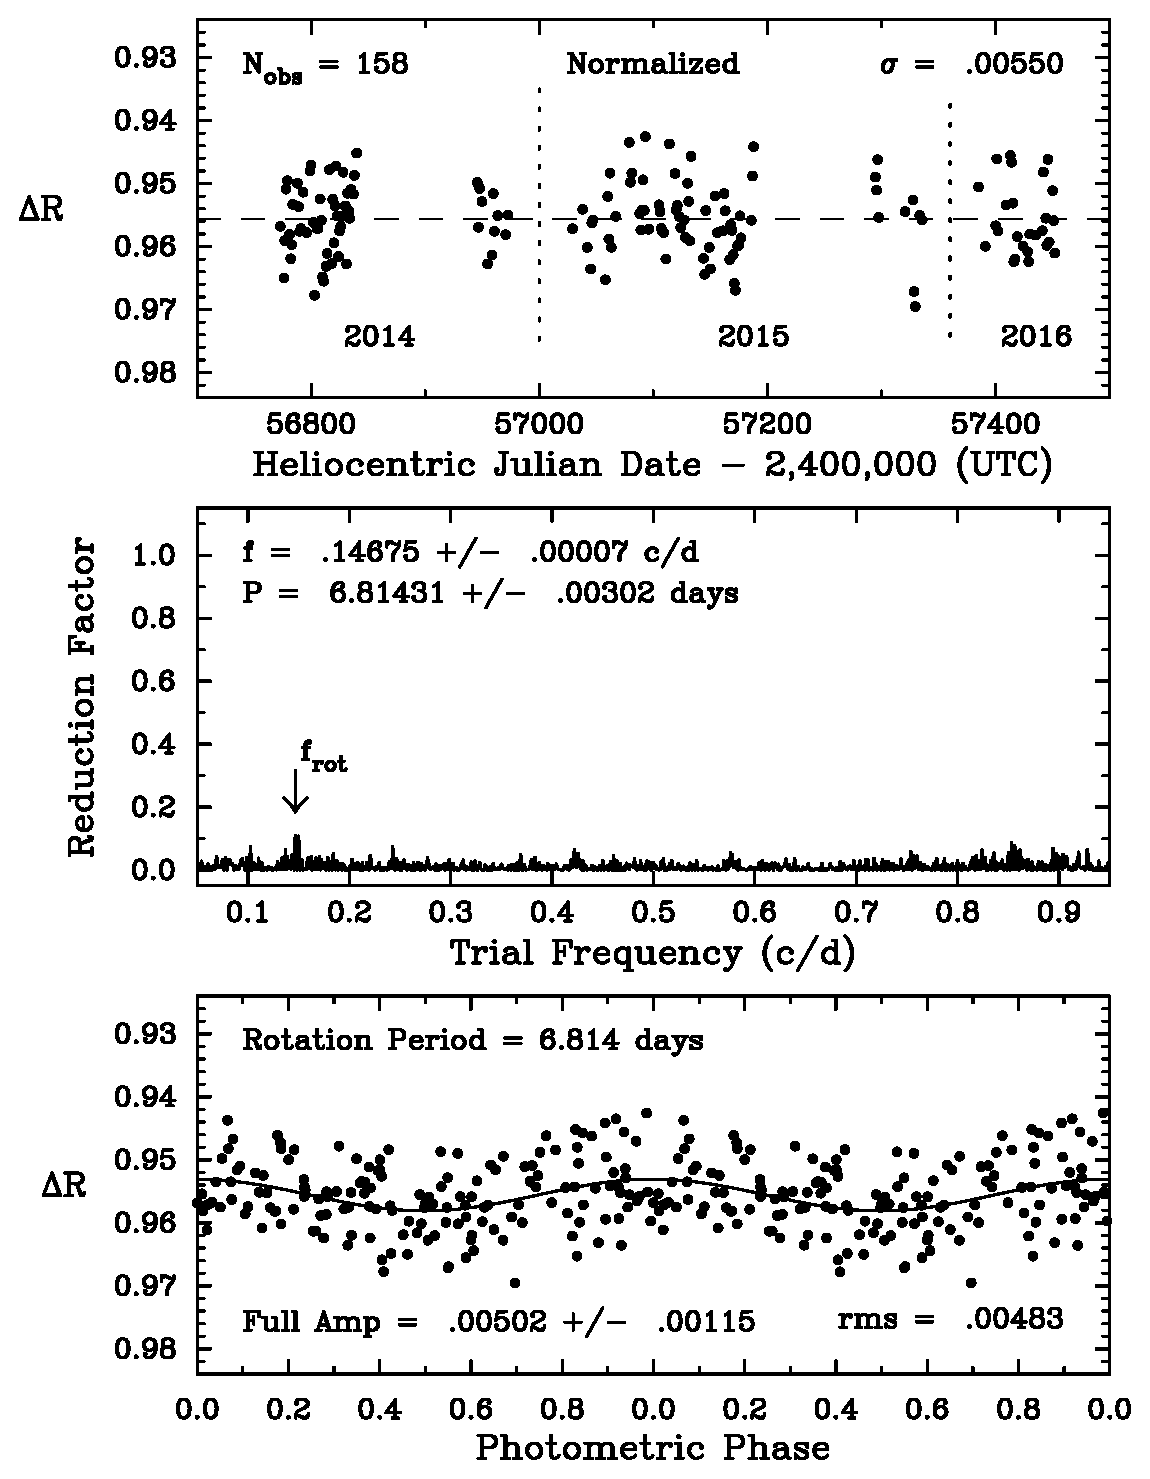
\includegraphics[width = 0.5\textwidth]{Figures/photometry.eps}
\caption{$Top$: The normalized nightly Cousins $R$ band photometric dataset for WASP-103, acquired with the C14 automated imaging telescope at Fairborn Observatory. Vertical dashed lines denote separate observing seasons. Gaps are due to target visibility and the Arizona monsoon season (July - September). $Middle$: The frequency spectrum of the normalized dataset suggests low-amplitude variability with a period of 6.814~days. $Bottom$: The normalized dataset phased to the 6.814-day period, which we interpret as the stellar rotation period. A least-squares sine fit to the 6.814-day rotation period gives a peak-to-peak amplitude of just 0.005~mag.}
\label{fig:photometry}
\end{figure}

\begin{deluxetable}{ccccc}
	%\tabletypesize{\small}
	\tablenum{1}
	\tablewidth{0pt}
	\tablecaption{Photometric Observations of WASP-103}
	\tablehead{
		\colhead{Observing} & \colhead{} & \colhead{Date Range} &
	\colhead{Sigma} & \colhead{Seasonal Mean} }% \\

%		\colhead{Season} & \colhead{$N_{obs}$} & \colhead{(HJD $-$ 2,400,000)} &
%		\colhead{(mag)} & \colhead{(mag)}}%   \\

	%	\colhead{(1)} & \colhead{(2)} & \colhead{(3)} &
	%	\colhead{(4)} & \colhead{(5)}  
	\startdata
	   2014   &  59 & 56722--56972 & 0.0057 & $0.9546\pm0.0007$  \\
	   2015   &  73 & 57028--57335 & 0.0062 & $0.9549\pm0.0007$  \\
	   2016   &  26 & 57385--57451 & 0.0055 & $0.9485\pm0.0011$  \\
	\enddata
	\label{tab:photometry}
\end{deluxetable}


\section{Light Curve Fits}
We fit a two-component model to the light curves. One component models the astrophysical signal (the planet's thermal phase variation and transit), and the other component models the systematic noise introduced by time-dependent changes in instrument performance. For each light curve, we fit the physical and systematic components simultaneously, such that the total observed flux as a function of time is given by $F(t) = F_\mathrm{physical}(t) \times F_\mathrm{sys}(t)$. For the \HST\ data, where we observed two phase curves and two additional eclipses, we constrain the physical parameters to be the same for all visits, but allow some of the systematics parameters to vary (for more details see \S\,\ref{sec:hst_sys}). We fit the WFC3 band-integrated (``white" light curve"), as well as the spectroscopic light curves (FIXME describe). 

\subsection{Astrophysical Signal}
We assume the astrophysical signal $F_\mathrm{physical}(t)$ has the following form:
\begin{equation}
	F_\mathrm{physical}(t) = T(t) \times P(t) \times E(t) 
\end{equation}
where $T(t)$ is the transit model, $P(t)$ is the thermal phase variation, $E(t)$ is ellipsoidal variation (change in the apparent radius of the planet with orbital phase due to tidal distortion), and $\alpha(\lambda)$ is the dilution from the companion star (FIXME).

We calculate the transit model with the \texttt{batman} package \citep{kreidberg15a}. The free parameters are the planet radius $r_p$, orbital inclination $i$, the ratio of semi-major axis to stellar radius $a/R_s$, and a linear stellar limb darkening parameter $u$.  We fixed the orbital period to $P = 0.925545613$ day and time of inferior conjunction to $t_0 = 2456836.2964455$, based on estimates from \cite{southworth15}.  We found that the system parameters were poorly constrained for the \HST/WFC3 phase curve (due to incomplete phase coverage) and \Spitzer\ Channel 1 phase curve (due to correlated noise), so for those light curves we fixed the the inclination to $i = 84.54^\circ$ and the semi-major axis to stellar radius $a/R_s  = 2.925$, based on the best fit to the \emph{Spitzer} Channel 2 light curve. (FIXME: looks like we used Southworth?)

We explored several different models for the planet's thermal phase variation $P(t)$, using climate maps from the open-source Python package \texttt{SPIDERMAN}. This package allows users to input a climate map (temperature or brightness as a function of latitude and longitude), and generate the corresponding thermal phase curve over a specified wavelength range. We tested three different maps:  a two-temperature map, with a uniform dayside temperature $T_d$ and a uniform nightside temperature $T_n$; a map generated with spherical harmonics; and the physically-motivated kinematic model from \cite{zhang16}, which has just three free parameters (the nightside temperature $T_n$, the change in temperature from day-to-night side $\Delta_T$, and the ratio of radiative to advective timescales $\xi$). These models each have different strengths. The kinematic model incorporates the most prior knowledge of physics, and even though it makes several simplifying assumptions (e.g, that the wind speed and direction are constant), it closely reproduces GCM simulations over a wide parameter space \citep{zhang16}.   The spherical harmonics map is the most flexible and makes the fewest assumptions about the true climate. The two-temperature model is the simplest and has the fewest free parameters.  In addition to these maps, we also fit the phase variation with a sinusoid, which has been used for many past analyses of exoplanet phase curves (FIXME).
%We explored adding an additional sine term to model the thermal phase variation, but the additional degrees of freedom are not justified according to the Bayesian Information Criterion (BIC). 

In addition to the changing temperature of the planet's surface, the visible surface area is also expected to change as a function of orbital phase.  WASP-103b is so close to its host star that it is likely tidally distorted and partially filling its Roche lobe \citep{gillon14}, which introduces ellipsoidal variations $E(t)$ in the light curve.  Our light curves are not precise enough to detect the ellipsoidal variability, but we include a model prediction $E(t)$ to avoid introducing any bias in the thermal phase variation. We model $E(t)$ using the analytic expression from \cite{leconte11}, which 

FIXME doppler beaming?

\begin{figure}
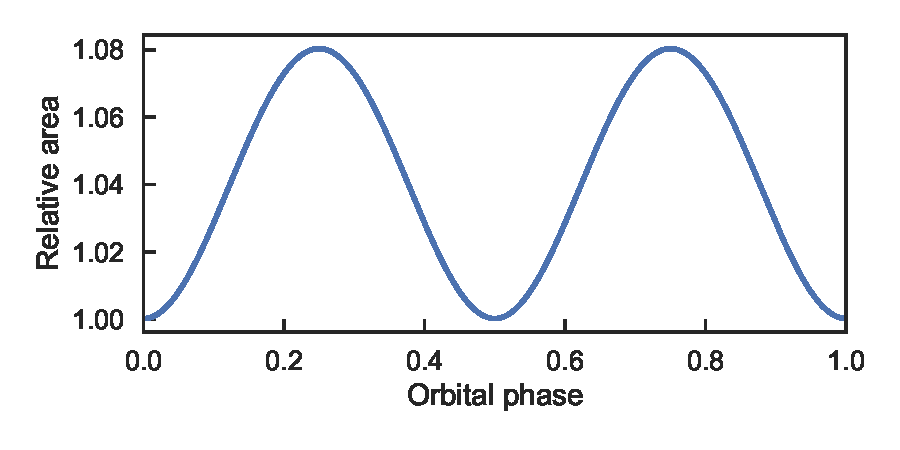
\includegraphics[width = 0.5\textwidth]{Figures/ellipsoidal.pdf}
\caption{Projected area of the planet as a function of orbital phase, normalized to unity at phase zero. The area variation was predicted analytically using the model from \citep{leconte11}.}
\label{fig:ellipsoidal}
\end{figure}


\subsection{Systematics}
Both the \HST\ and \Spitzer\ phase curves have systematic noise caused by variations in the sensitivity of the instrument over time. For the \HST/WFC3 data, the dominant systematic is an orbit-long exponential trend due to charge traps filling up over successive exposures \citep{long15, zhu17}. For \Spitzer\, the primary source of noise is the intrapixel sensitivity effect. The detector's pixels do not have uniform sensitivity, so slight changes in telescope pointing cause the recorded flux to vary. 

\subsubsection{\HST\ Systematics}
\label{sec:hst_sys}
We fit the WFC3 systematics using an analytic model of the form:
\begin{equation}
 F_\mathrm{sys}(t) = (c\,S(t) + v_1\,t_\mathrm{v} + v_2\,t_\mathrm{v}^2)(1 - \exp(-a\,t_\mathrm{orb} - b))
\end{equation}
where $t_\mathrm{v}$ is time elapsed since the first exposure in a visit and $t_\mathrm{orb}$ is time since the first exposure in an orbit. $S(t)$ is a scale factor equal to 1 for exposures with spatial scanning in the forward direction and $s$ for reverse scans, to account for the upstream-downstream effect (FIXME). The orbit-long ramp parameters are consistent for all the visits, so we constrained $a$, $b$, and $s$ to have the same value for all visits in the final fit. The visit-long trends differ from visit to visit, so $c$, $v_1$, and $v_2$ were allowed to vary between visits. We fixed $v_2$ to zero for the two secondary eclipse observations from Program 13360, since the visit-long trend for shorter observations is fit well by a linear slope.

Some segments of the data exhibit stronger systematics than others, so we exclude these data in our final analysis. We drop the first orbit from every visit and the first exposure from every orbit \citep[following common practice; see e.g.][]{kreidberg14a}.  We also discard exposures from the last half of orbit 15 from the phase curve observations, which were taken in staring mode to enable a gyro bias update. Since we observed two phase curves, we have complete orbital phase coverage the planet despite discarding some data.

\subsubsection{\Spitzer\ Systematics}
We fit the \Spitzer\ systematics with the BLISS mapping technique \citep{stevenson12}. This technique creates a map of the intrapixel sensitivity while simultaneously fitting for other systematics and the physical parameters of the system. In addition to the intrapixel sensitivity map, we fit the data for a linear trend in time. 

\begin{figure}
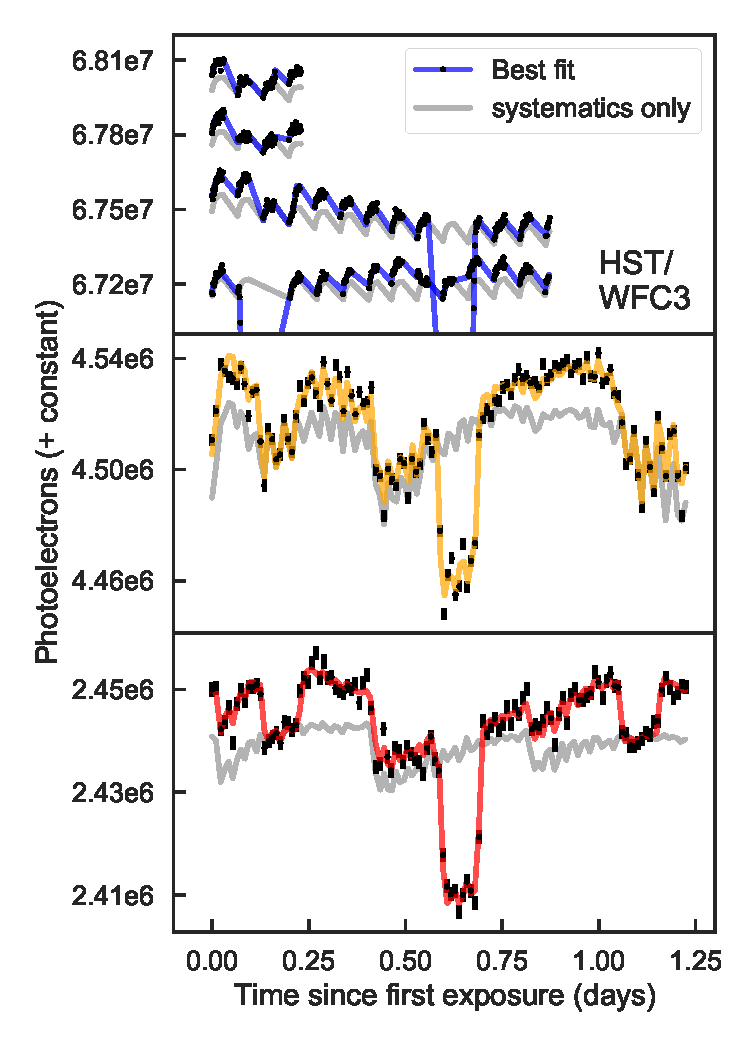
\includegraphics[width = 0.5\textwidth]{Figures/systematics.pdf}
\caption{Raw light curves for WASP-103b observed with \HST/WFC3 (top panel) and \Spitzer/IRAC (bottom two panels). The data points are indicated with black dots. The \HST\ data are unbinned, and the Spitzer data are binned in time segments of FIXME minutes with error bars indicating the bin standard deviation. The colored lines show the best fit models, which include the astrophysical signal and instrument systematics. The gray lines indicate the contribution from the instrument systematics alone (which would be observed for a source with constant brightness and no planet). For visual clarity, we corrected the \HST\ data for the upstream-downstream effect, separated the four visits by adding a flux offset, and zoomed in on the phase variation, so the transits are not displayed in the panel.}
\label{fig:systematics}
\end{figure}


\section{Results}
We achieved good quality fits!

\begin{figure}
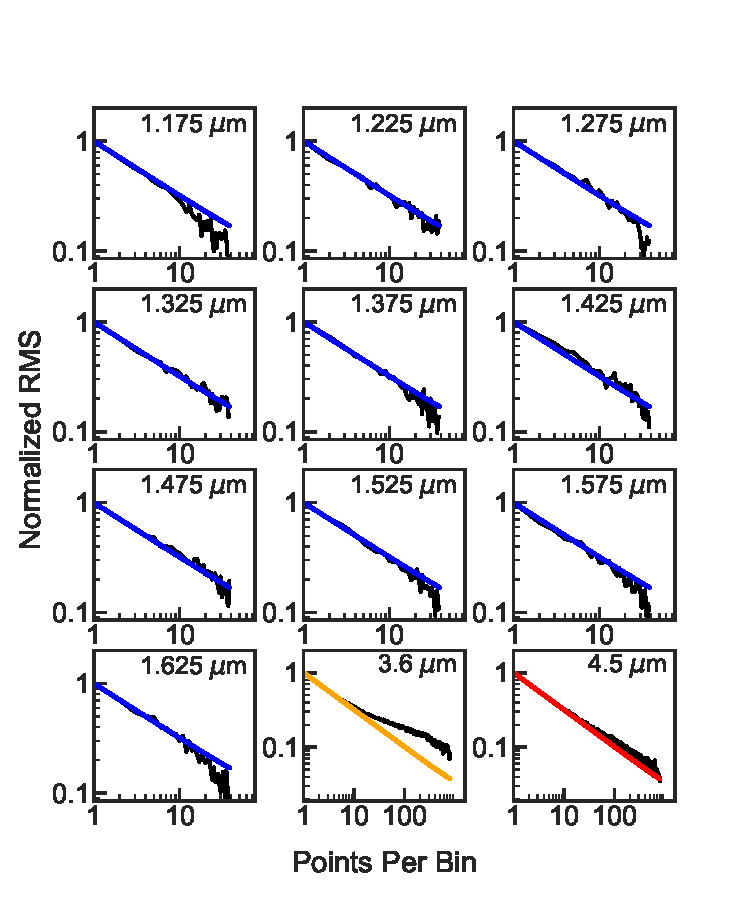
\includegraphics[width = 0.5\textwidth]{Figures/rms.pdf}
\caption{Root mean square (rms) variability in the light curves as a function of bin size (black lines) compared to the expected rms from photon noise (colored lines). The central wavelength of the light curve is indicated in the upper right corner of each panel. With the exception of the \Spitzer\ 3.6 $\mu$m channel, the rms for the light curves bins down in agreement with predictions from the photon noise.}
\label{fig:rms}
\end{figure}

\begin{figure*}
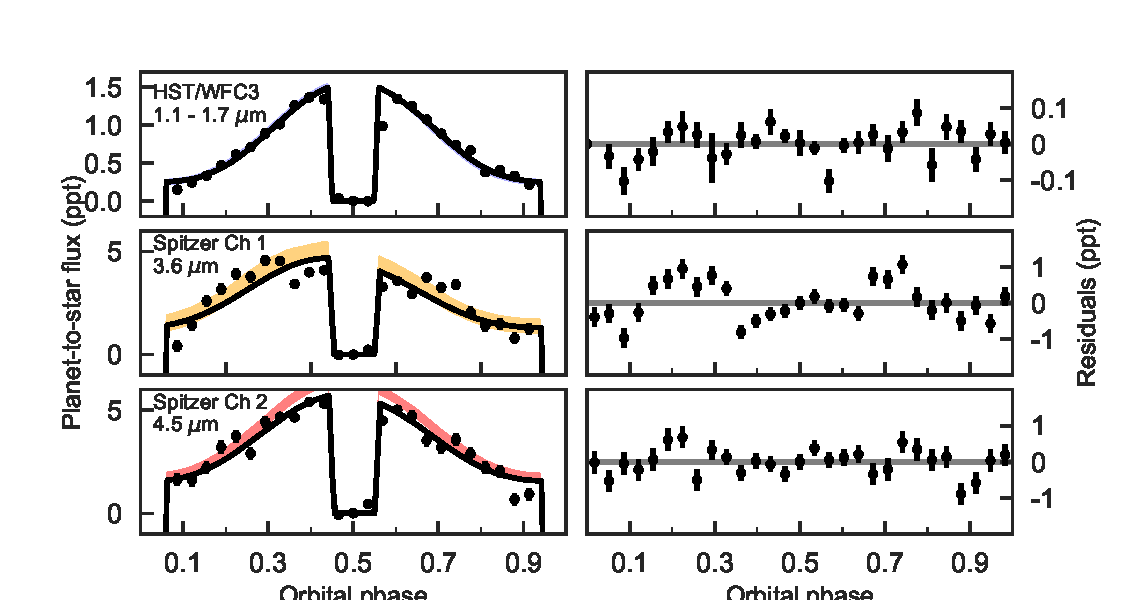
\includegraphics[width = 1.0\textwidth]{Figures/phase_curves.pdf}
\caption{WASP-103b phase curve observations from \HST/WFC3 (top) and \Spitzer/IRAC (middle and bottom). For clarity, the data are phase-folded on the planet's orbital period and binned in 30 uniformly spaced bins between 0 and 1. The left column shows the phase curves with systematic noise removed (black points) compared to the best fit model (black line). The shading denotes the  1\,$\sigma$ confidence interval on the best fit. We include the transits in the fit, but they are not displayed in this figure. The right-hand column shows the binned residuals for the best-fit light curve.}
\label{fig:phasecurves}
\end{figure*}

\subsection{Phase-Resolved Spectra}
We used the best-fit phase curves (with systematics removed) to generate phase-resolved emission spectra. We binned each phase curve in FIXME evenly spaced intervals between phase FIXME and FIXME. In each phase bin, we estimated the planet-to-star flux by taking the mean value of the data points in the bin. To estimate the uncertainty, we took the standard deviation of the points in the bin and added it in quadrature to the standard deviation of the data points during secondary eclipse (phase FIXME to FIXME). This procedure accounts for the uncertainty in the baseline stellar flux (which we measure during secondary eclipse).

To estimate the dayside planet-to-star flux, we did FIXME.

We note that the phase-resolved spectra do not significantly change based on which model we assume for the  

\subsection{Comparison of Thermal Phase Variation Models}
All four of the thermal phase variation models we consider (two-temperature, kinematic, spherical harmonics, and sinusoid) provide good fits to the observed phase curves. Table FIXME summarized the goodness of fit

\subsection{Hotspot Offset}

\section{Retrieval}

\subsection{Bond Albedo}

\section{Comparison with GCMs}

\section{Comparison with Brown Dwarfs and Directly Imaged Planets}
cite Tremblin et al. 2017 ? (https://arxiv.org/pdf/1710.02640.pdf)

\section{Discussion and Conclusions}

\acknowledgments
We thank a lot of people. Caroline Morley, Thomas Beatty, Ming Zhao, Kim Star Cartier, Hannah Diamond-Lowe, Nick Cowan (make him a coauthor?)

\bibliographystyle{aasjournal}
\bibliography{ms.bib}

\end{document}

